\documentclass[tikz]{standalone}

\usetikzlibrary{shapes}
\usetikzlibrary{calc} 

\usetikzlibrary{decorations.pathreplacing}
\usetikzlibrary{decorations.markings}
\usetikzlibrary{decorations.pathmorphing}
\usetikzlibrary{decorations.text}

\usepackage{mathtools}
\providecommand\enpos[2]{\underset{\footnotesize\mathbf{\mathclap{\left\lfloor#1,#2\right\rceil}}}{N}}

% This bascially automates a \newcommand{<name>}{} to ensure
% that a command with the given <name> does not already exist
\providecommand*{\pgfmathsetnewmacro}[2]{%
    \newcommand*{#1}{}% Error if already defined
    \pgfmathsetmacro{#1}{#2}%
}%

\begin{document}

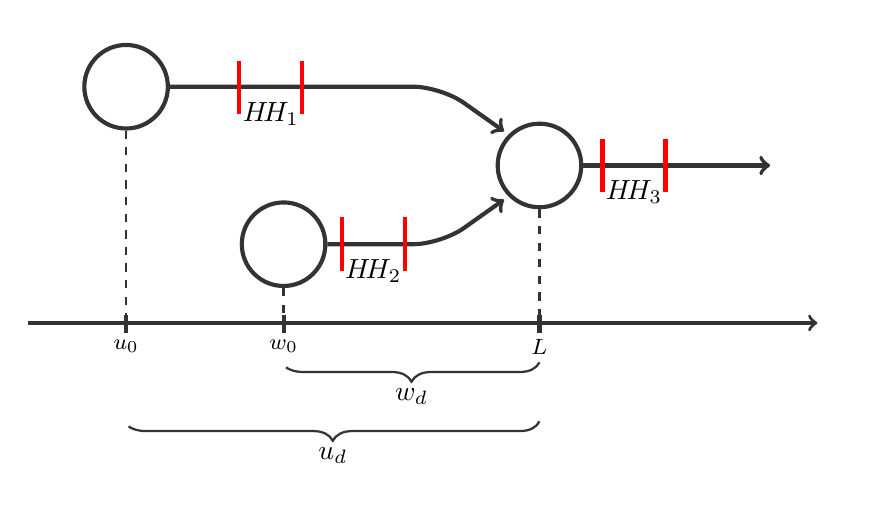
\begin{tikzpicture}[%
        scale = 1,
        draw = black!80,
        fill = white,
        line width = 1.5pt,
        shorten >=2pt,
        % decoration={random steps, amplitude = 0.25cm, segment length=0.8cm},
        % smooth
        ]


\useasboundingbox[clip] (-5.25,-4) rectangle (5.25,2);

\pgfmathsetnewmacro{\nipos}{-4}
\pgfmathsetnewmacro{\niipos}{-2}
\pgfmathsetnewmacro{\niiipos}{1.25}


\draw[line width = 1.2pt,->] (-5.25,-1.75) -- (4.85,-1.75);
% \draw[line width = 1.2pt,->] (-4.75,-2.25) -- (-4.75,1.95);

\coordinate (d1) at (\nipos, -1.75);
\coordinate (d2) at (\niipos, -1.75);
\coordinate (d3) at (\niiipos, -1.75);

\begin{scope}[rounded corners = 10pt,yshift = 0.25cm]
    \node (N1) [circle, draw, fill = white] at (\nipos,1) 
        {\large \phantom{$\enpos{1}{0}$}%
        };
    \node (N2) [circle, draw, fill = white] at (\niipos,-1)
        {\large \phantom{$\enpos{1}{1}$}%
        };
    
    \node (N3) [circle, draw, fill = white] at (\niiipos,0)
        {\large \phantom{$\enpos{2}{0}$}%
        };
    
    \draw[->,decorate] (N1) -- (0,1) -- (N3.north west);
    \draw[->,decorate] (N2) -- (0,-1) -- (N3.south west);
    
    \draw[->,decorate] (N3) -- +(0:3);
    
\end{scope}

\foreach \INDEX in {1,2,3}{%
    \draw[dashed, line width = 0.8pt] (N\INDEX) -- (d\INDEX);
    }

\foreach \POSI/\NAME in {d1/$u_0$,d2/$w_0$,d3/$L$}{%
    \draw (\POSI)+(0,0.1) -- +(270:0.2);
    \node[anchor = north, yshift = -2pt] at (\POSI) {\footnotesize\NAME}; 
    }
    
\node (a) [fill] at ($(N1)!0.35!(N3)$) {$H\!H_1$};
\foreach \SIGN in {+,-}{
    \path (a) -- +(90\SIGN90:0.4cm) coordinate (a\SIGN);
    \draw[red] (a\SIGN) -- +(90:0.75);
    }


\node (b) [fill, anchor = north,yshift = -0.4cm] at ($(N2)!0.35!(N3)$) {$H\!H_2$};
\foreach \SIGN in {+,-}{
    \path (b) -- +(90\SIGN90:0.40cm) coordinate (b\SIGN);
    \draw[red] (b\SIGN) -- +(90:0.75);
    }

\node (c) [fill, anchor = north, yshift = 0.05cm] at ($(N3)!0.4!(\niiipos+3,0)$) {$\mathclap{H\!H_3}$};
\foreach \SIGN in {+,-}{
    \path (c) -- +(90\SIGN90:0.4cm) coordinate (c\SIGN);
    \draw[red] (c\SIGN) -- +(90:0.75);
    }

\draw[decoration ={brace, amplitude = 7, raise = 0.50cm}, decorate, line width = 0.8pt] (d3) -- (d2) node[midway, anchor=north,yshift =-0.70cm] {$w_{\scriptsize d}$};
\draw[decoration ={brace, amplitude = 7, raise = 1.25cm}, decorate, line width = 0.8pt] (d3) -- (d1) node[midway, anchor=north,yshift =-1.45cm] {$u_{\scriptsize d}$};
    

\end{tikzpicture}

\end{document}